\subsection{Session 2, Exercise 06}

\lineparagraph{Exercise}

Perform the following for both nondeterministic finite automata.
\begin{enumerate}[a.)]
    \item Give the computation tree of word $baabab$.
    \item Create an equivalent DFA by the procedure studied in class.
    \item Which languages are recognized by these automata?
\end{enumerate}

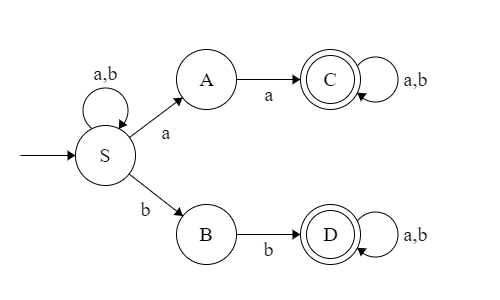
\includegraphics[width=0.5\linewidth]{02/2_6_1_automaton.png}

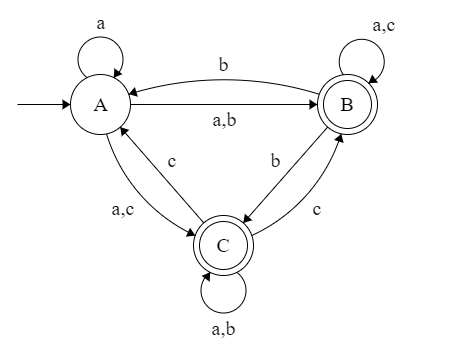
\includegraphics[width=0.5\linewidth]{02/2_6_2_automaton.png}

\lineparagraph{Solution}

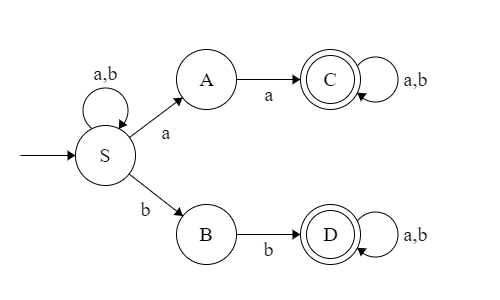
\includegraphics[width=0.5\linewidth]{02/2_6_1_automaton.png}

Give the computation tree of word $baabab$:

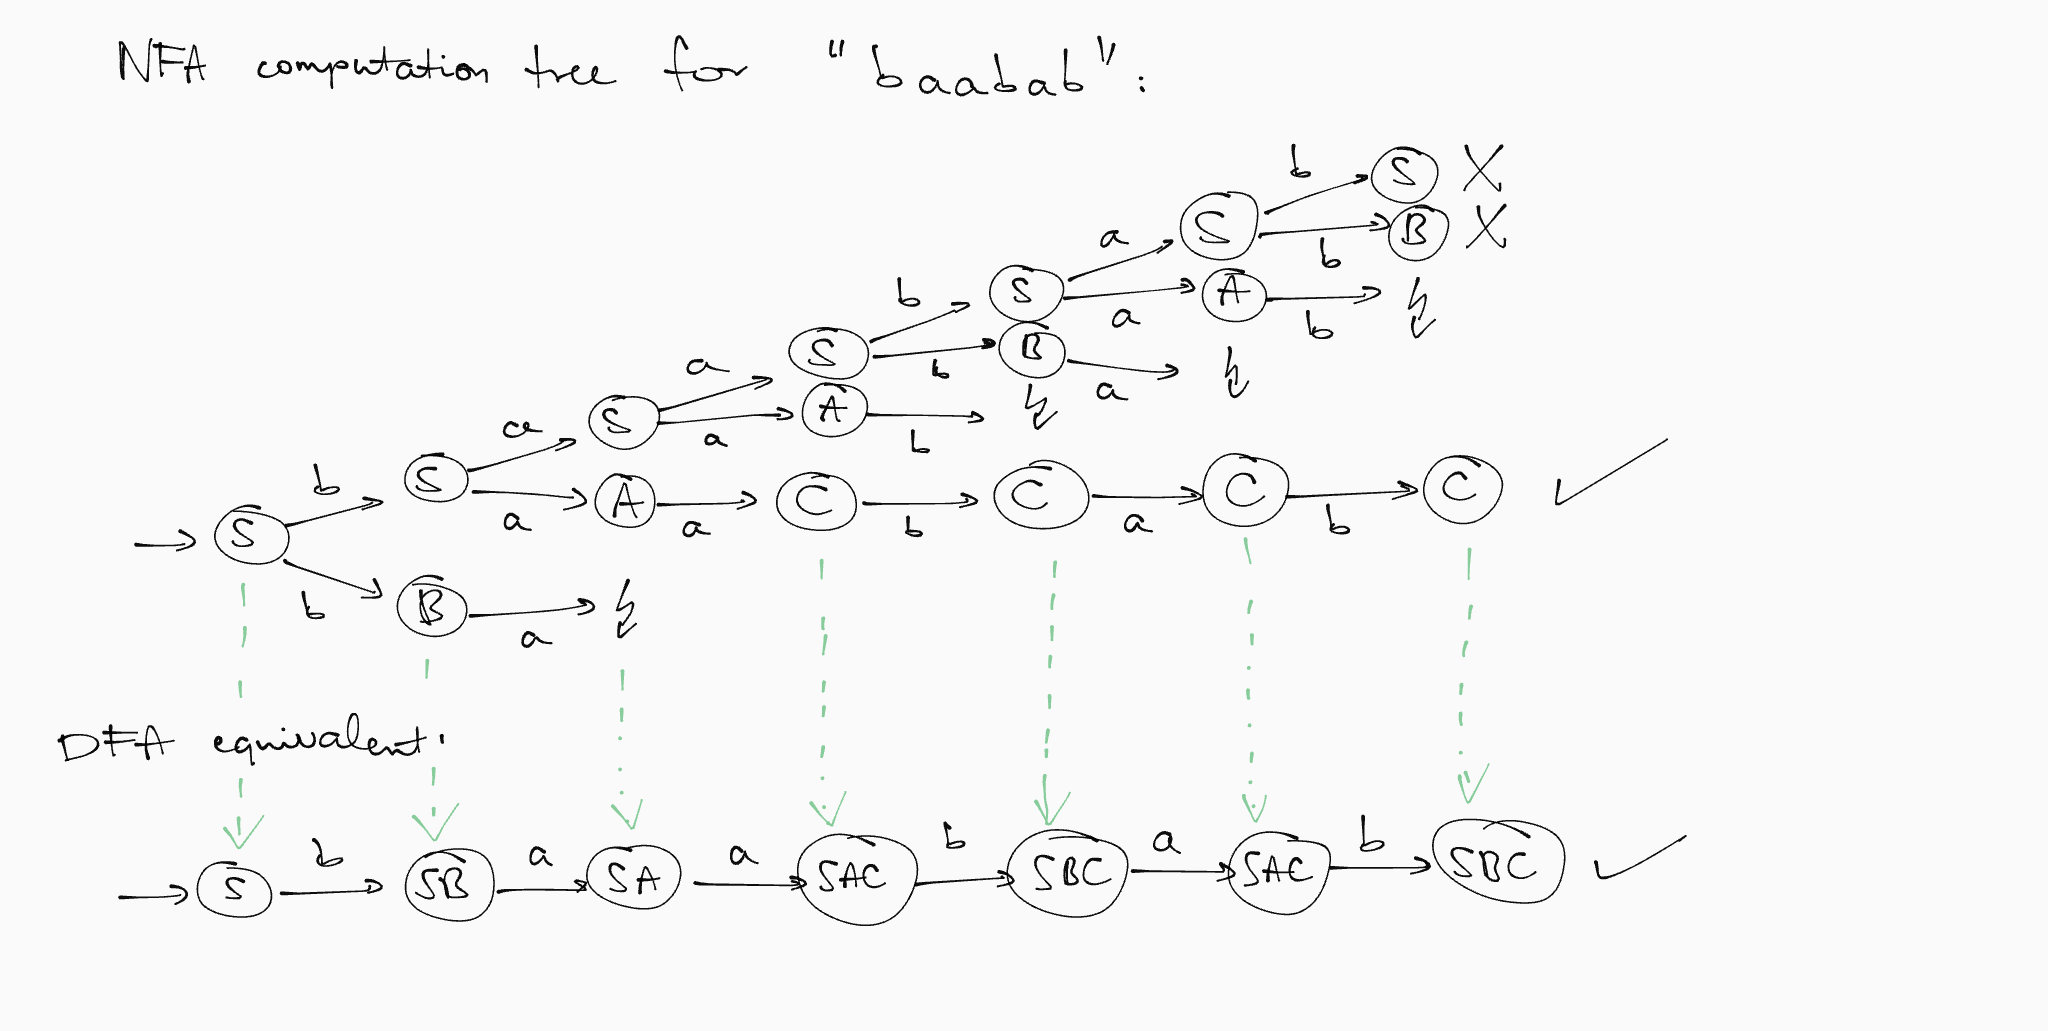
\includegraphics[width=\linewidth]{02/comp_tree_1_nfa_dfa.png}

The word $baabab$ is accepted, since there exists a branch that resulted in an accept state ($C$).

The DFA equivalent computation is also shown in the drawing. We basically follow all branches in ''parallel'', using meta states. We will construct the DFA, that will do a computation like this one:

\textbf{Step 1}

We start with the same starting state as in the NFA: $S$.

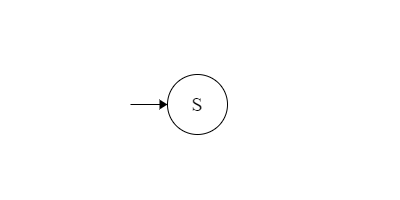
\includegraphics[width=0.5\linewidth]{02/dfa_step_01.png}

\textbf{Step 2}

Then, we check where can we move for an $a$ input from $S$ in the NFA: $S\xrightarrow{a}\{S,A\}$, so we add the $SA$ state for an $a$ transition, and similarly for $S\xrightarrow{b}\{S,B\}$, so we add the $SB$ state for a $b$ transition.

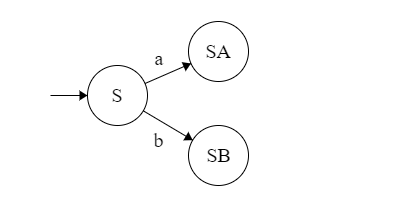
\includegraphics[width=0.5\linewidth]{02/dfa_step_02.png}

Check back on the DFA equivalent on the drawing above! You will notice the state $SB$ as the second step.

\textbf{Step 3}

And we continue the same thing for the new states:

Where does $SA$ move for an input character of $a$? The transitions from $S$ and from $A$ for input $a$ are: $S\xrightarrow{a}\{S,A\}$ and $A\xrightarrow{a}\{C\}$, so together they move to state $SAC$.

Where does $SA$ move for an input character of $b$? The transitions from $S$ and from $A$ for input $b$ are: $S\xrightarrow{b}\{S,B\}$ and $A\xrightarrow{b}\{\}$, so together they move to state $SB$.

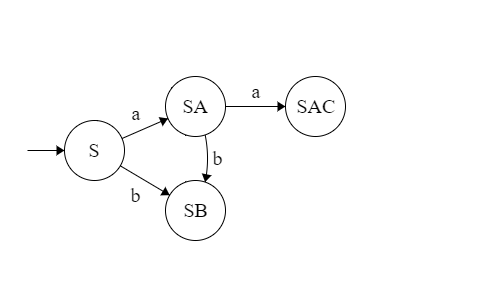
\includegraphics[width=0.7\linewidth]{02/dfa_step_03.png}

The process is the same: find a state that does not have all transitions defined (for $a$ and for $b$ input as well), check where their basis states transition in the NFA for the given input and add it as a transition. If the resulting state does not exist, add the state.

When no new states are added and all states transitions are fully defined the process is done.

\textbf{Step 4}

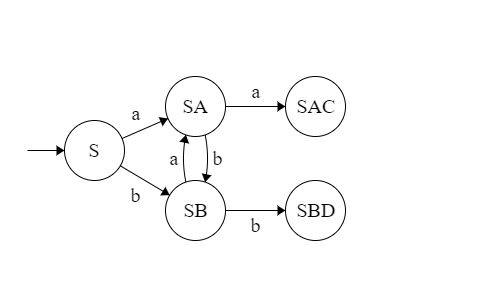
\includegraphics[width=0.7\linewidth]{02/dfa_step_04.png}

\textbf{Step 5}

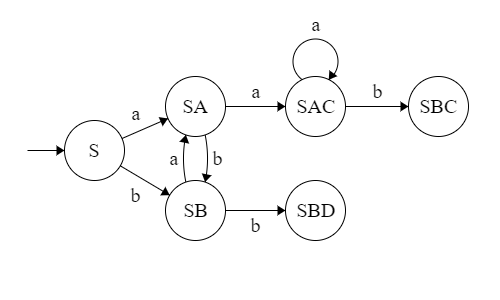
\includegraphics[width=0.7\linewidth]{02/dfa_step_05.png}

\textbf{Step 6}

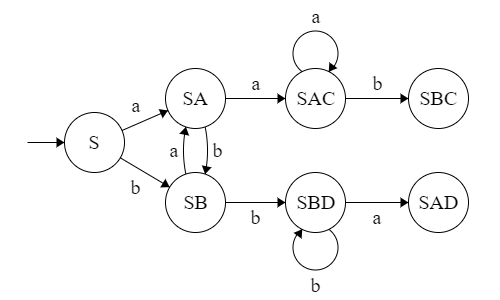
\includegraphics[width=0.7\linewidth]{02/dfa_step_06.png}

\textbf{Step 7}

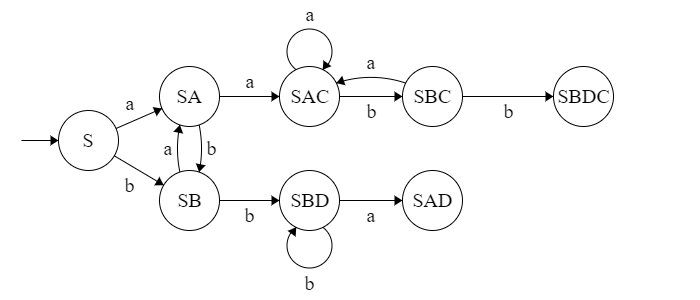
\includegraphics[width=0.9\linewidth]{02/dfa_step_07.png}

\textbf{Step 8}

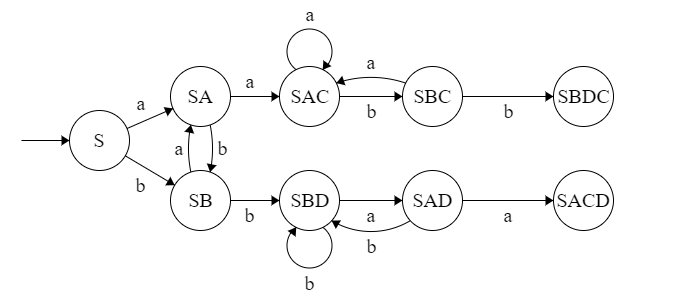
\includegraphics[width=0.9\linewidth]{02/dfa_step_08.png}

\textbf{Step 9}

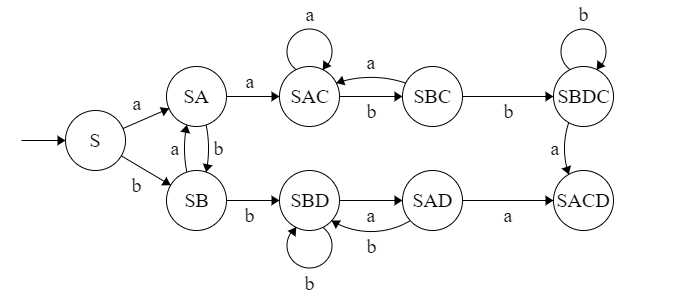
\includegraphics[width=0.9\linewidth]{02/dfa_step_09.png}

\textbf{Step 10}

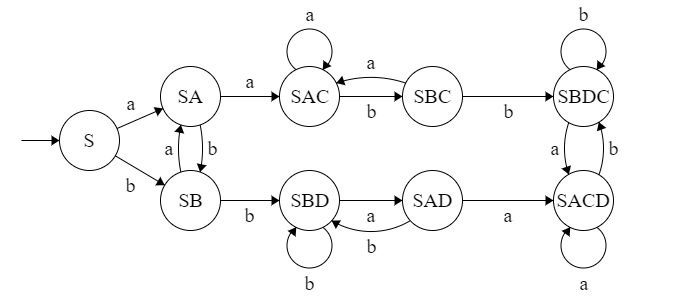
\includegraphics[width=0.9\linewidth]{02/dfa_step_10.png}

\textbf{Step 11}

Finally, define the accepts states: Any state that contains an original accept state (in this case $C$ or $D$) will be an accepting state:

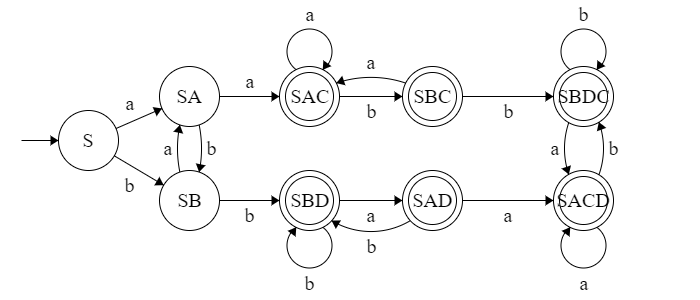
\includegraphics[width=0.9\linewidth]{02/dfa_step_11.png}

\textbf{Note}

By the way, the automaton can be simplified, like this:

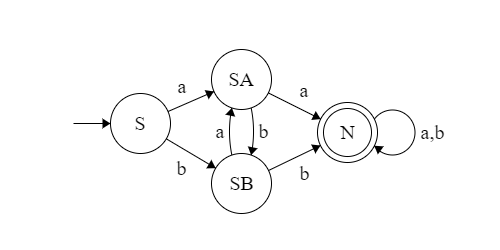
\includegraphics[width=0.7\linewidth]{02/dfa_final.png}

Since the moment we reach any of the accepts states, we will never leave them.


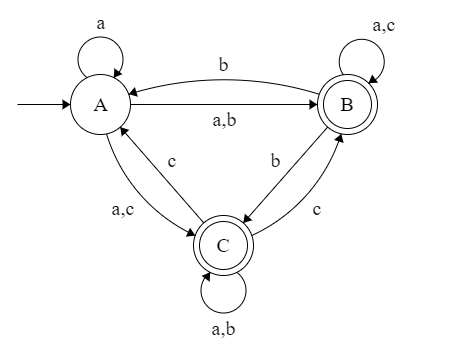
\includegraphics[width=0.5\linewidth]{02/2_6_2_automaton.png}

TODO